\documentclass[landscape]{article}
\usepackage[utf8]{inputenc}
\usepackage[T1]{fontenc}
\usepackage{microtype}
\usepackage{newspaper}
\usepackage{sudoku}
\usepackage{booktabs}

\date{\today}
\currentvolume{1}
\currentissue{1}

\SetPaperName{The Daily Hennig}
\SetHeaderName{The Daily Hennig}
\SetPaperLocation{Somerville, MA}
\SetPaperSlogan{``All the News I Feel Like Printing.''}
\SetPaperPrice{Zero Dollars}

\usepackage{graphicx}
\usepackage{multicol}
\usepackage{picinpar}
\usepackage{newspaper-mod} % modifies newspaper style

\setlength\textwidth{9.5in}		% article default = 418pt
\setlength\textheight{7.0in}		% article default = 296pt

%%%%%%%%%  Front matter   %%%%%%%%%%

\usepackage{lipsum}
\renewcommand\headline[1]{\begin{center} {\huge \textsl{ #1}}\\ %
			\rule[5pt]{0.8\hsize}{0.5pt}\\ \end{center}}

\begin{document}
\maketitle

\begin{multicols}{3}
\headline{Weather}

\center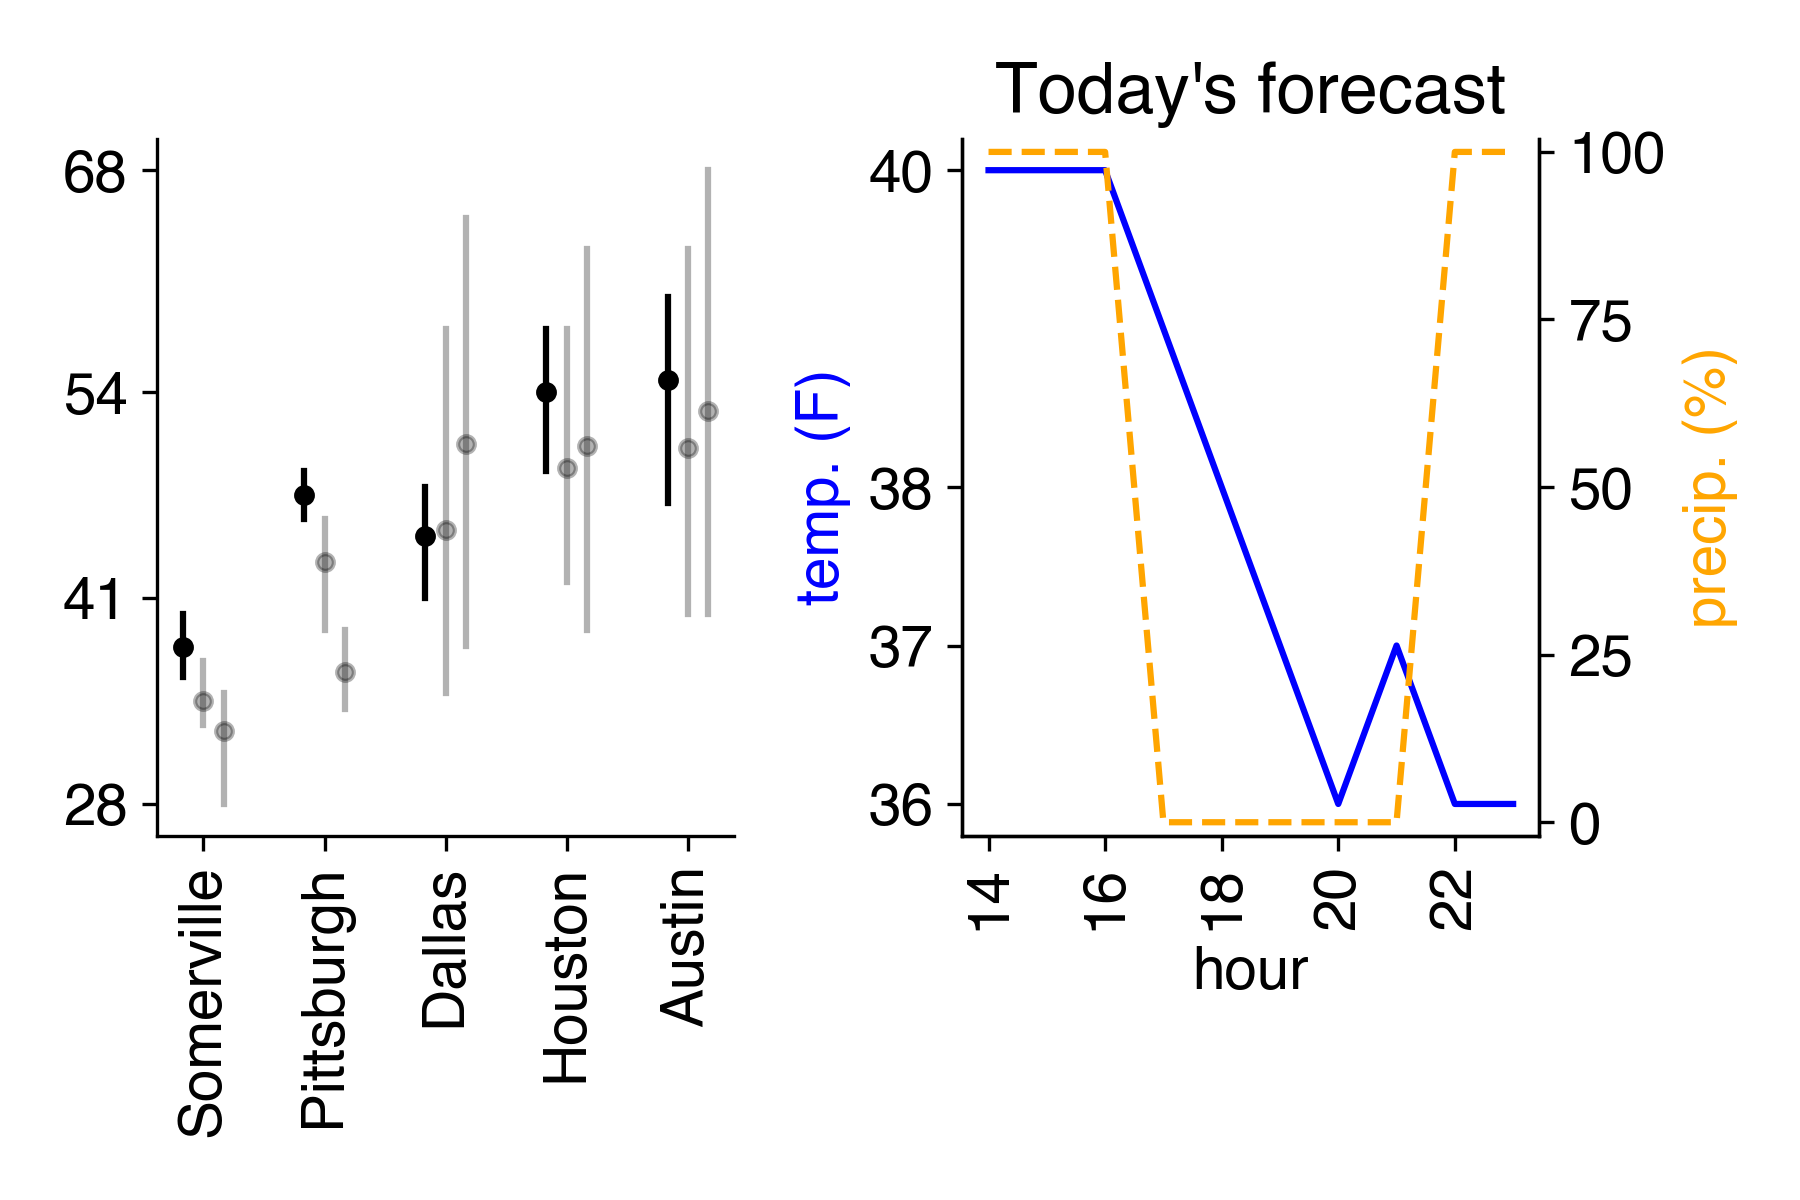
\includegraphics[width=\linewidth]{images/weather.png}

% \columnbreak

\headline{Sports}

\begin{center}
	NBA games last night:
\begin{tabular}{llll}
\toprule
     Boston & 116 &  Houston & 107 \\
LA Clippers & 125 & Brooklyn & 114 \\
  LA Lakers & 134 & Portland & 110 \\
    Orlando & 105 &    Miami &  87 \\
\bottomrule
\end{tabular}

\end{center}
\begin{center}
	\textbf{NHL games last night:
}\begin{tabular}{llll}
\toprule
       Dallas Stars & 4 &     Anaheim Ducks & 3 \\
      Boston Bruins & 3 &   Ottawa Senators & 2 \\
Carolina Hurricanes & 3 & New Jersey Devils & 2 \\
\bottomrule
\end{tabular}

\textbf{Boston Bruins}

Record: 30-9-9 (69 points), 1st in NHL Atlantic 

Next Game: Saturday, Jan. 27 vs. PHI
\end{center}

\headline{Games}
% \vspace{-1cm}
\center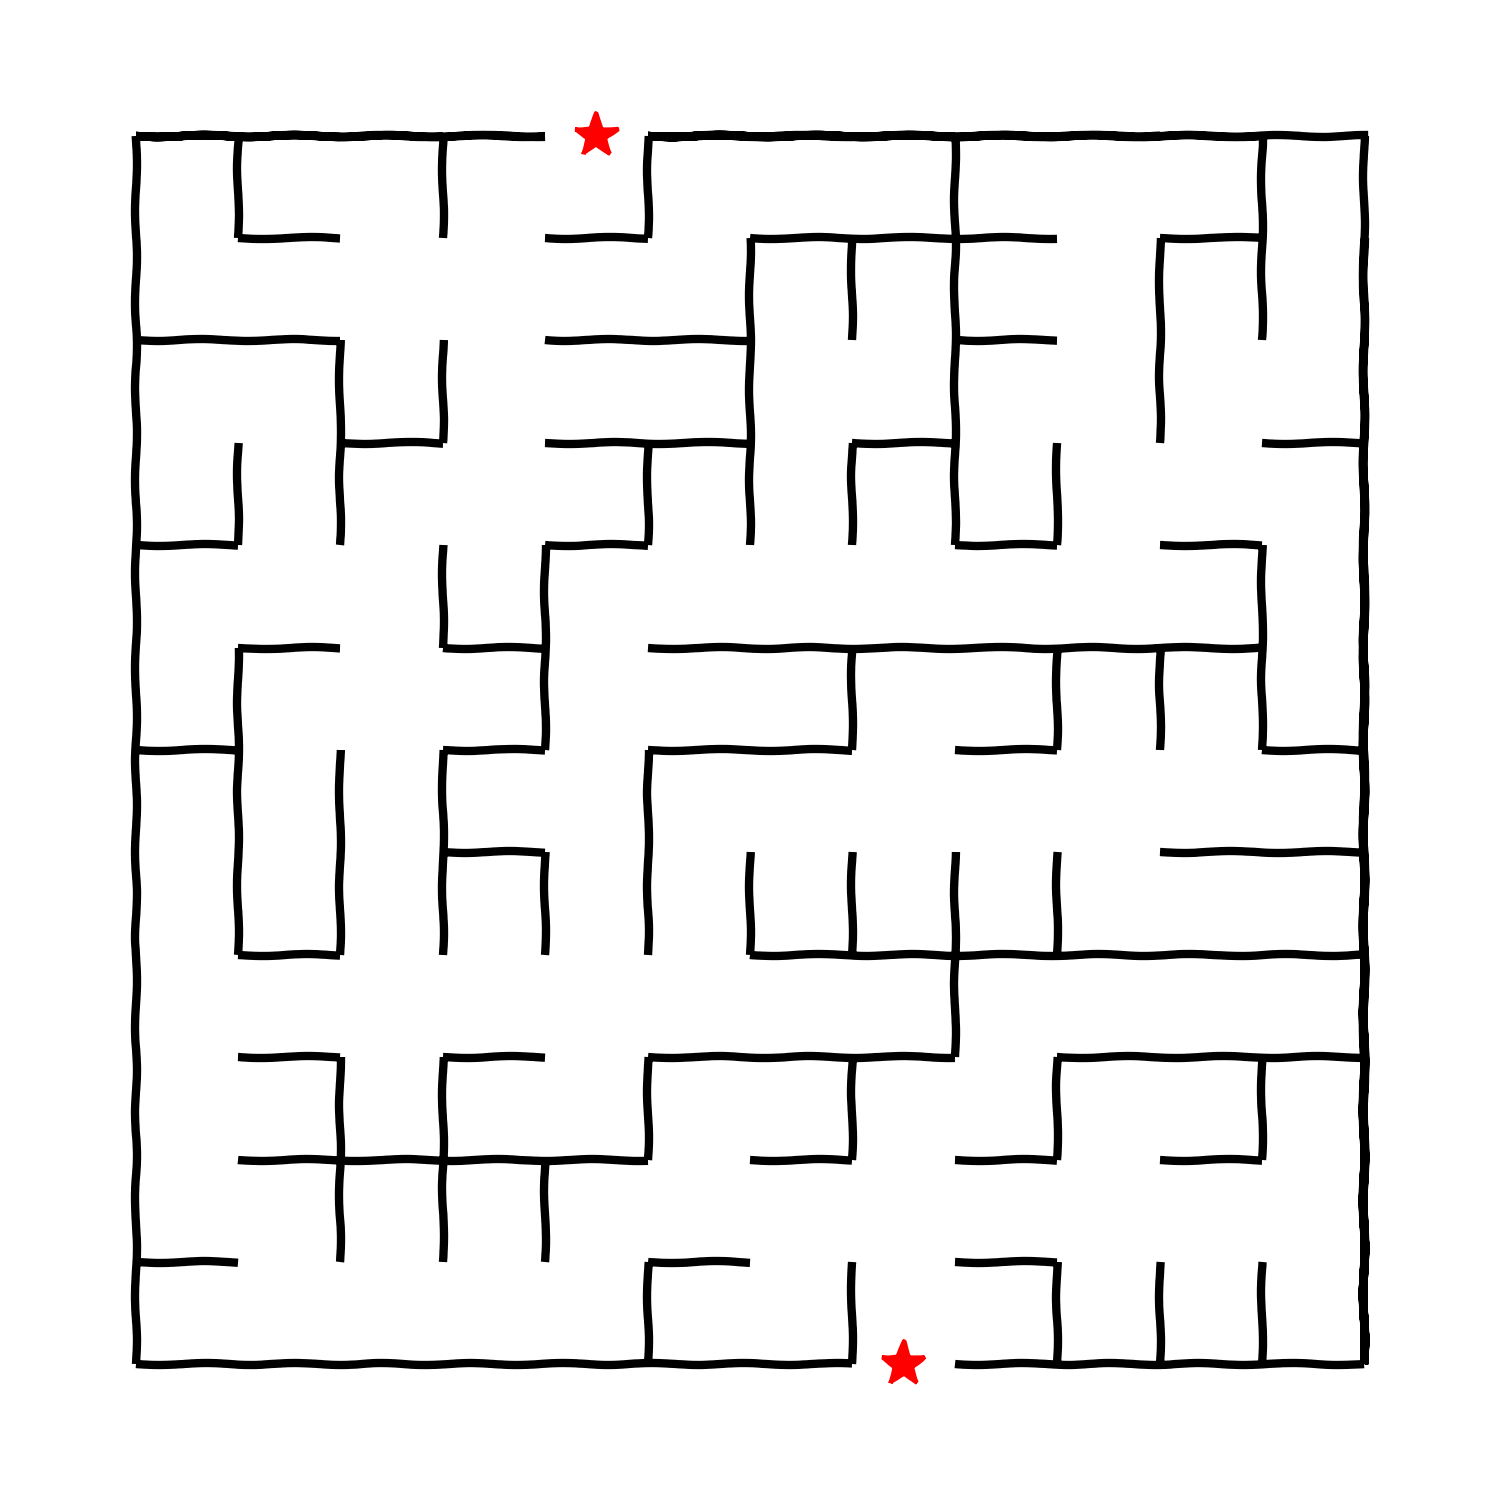
\includegraphics[width=0.49\linewidth]{images/maze_r.png}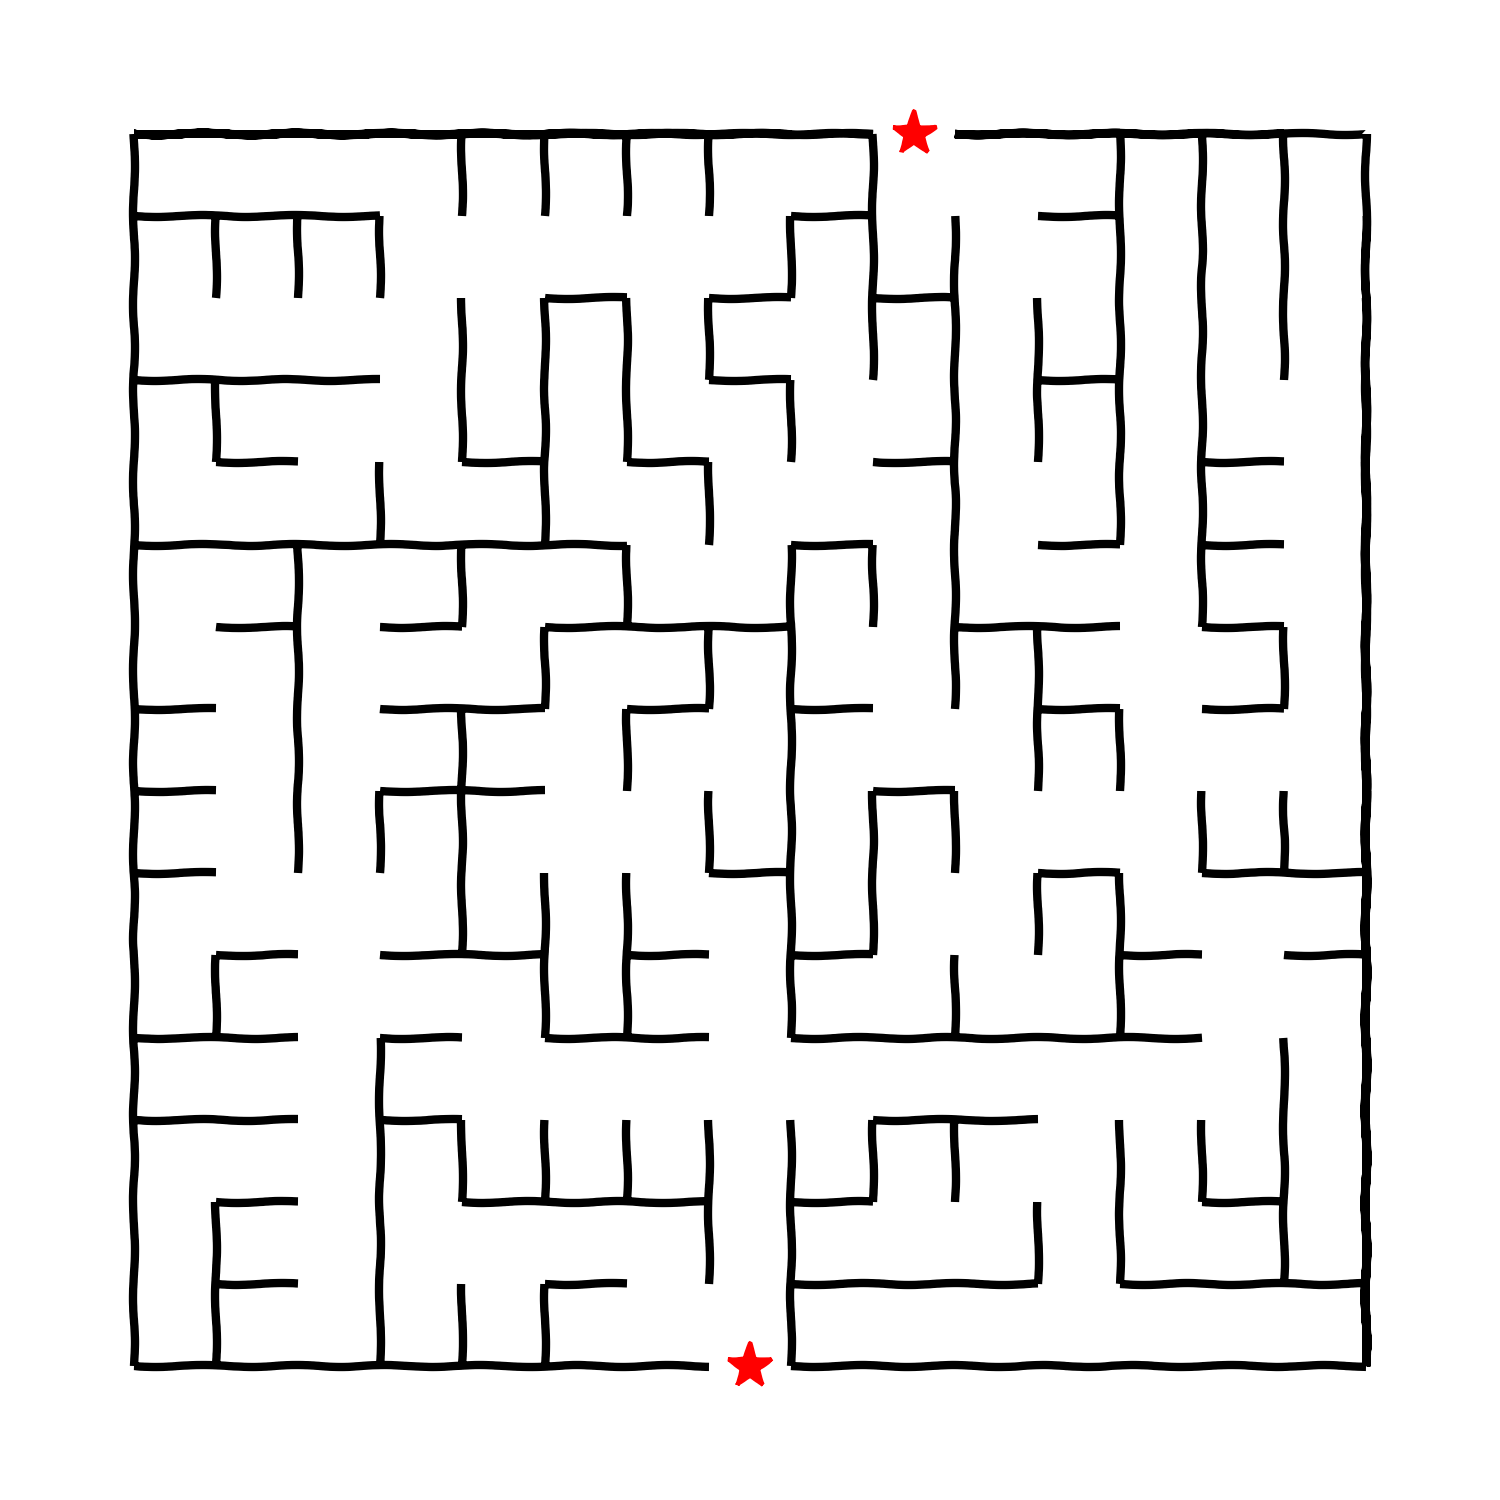
\includegraphics[width=0.49\linewidth]{images/maze_j.png}

\renewcommand*\sudokuformat[1]{\sffamily#1}
\setlength\sudokusize{4cm}
\setlength\sudokuthickline{1pt}
\begin{center}
	\begin{sudoku-block}| | | | | |2|9| | |.
| |4| |7| | |5| | |.
|8|7|9| | | | | | |.
| | | | |8| | |4| |.
|7| |8| |2| | | |6|.
| |1| | | | | |7| |.
|6| | |8| | |1|3| |.
| | | | | |3|4|6| |.
| |2|1|5|4| | | | |.
\end{sudoku-block}
\end{center}

\columnbreak
\headline{Comics}
% \vspace{-1.5cm}
\center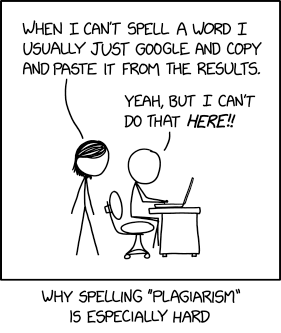
\includegraphics[width=0.5\linewidth]{images/comic-xkcd.png}
\center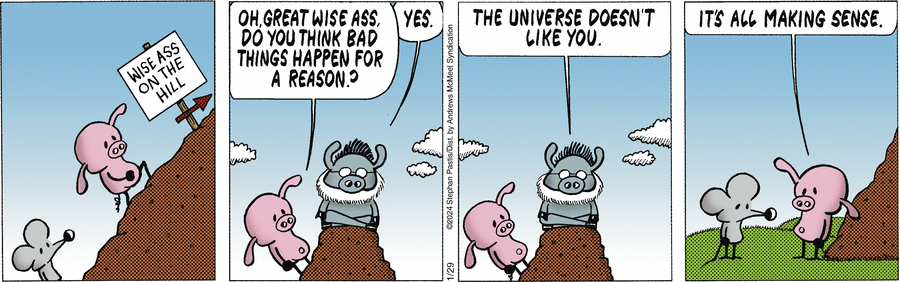
\includegraphics[width=\linewidth]{images/comic-pearls.png}
\center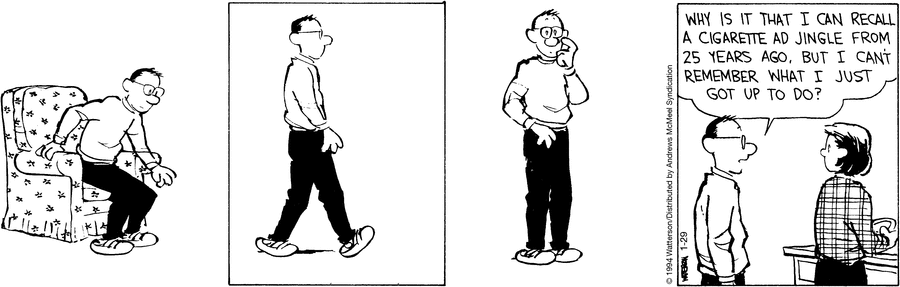
\includegraphics[width=\linewidth]{images/comic-calvinandhobbes.png}

\end{multicols}

\end{document}